\documentclass[12pt]{article}
\usepackage[utf8]{inputenc}
\usepackage{geometry}
\usepackage{graphicx}
\usepackage{listings}
\usepackage{xcolor}
\usepackage{amsmath}
\usepackage{amsfonts}
\usepackage{amssymb}
\usepackage{fancyhdr}
\usepackage{titlesec}
\usepackage{url}
\usepackage{float}
\usepackage{hyperref}

% Set page margins
\geometry{a4paper, left=0.8in, right=0.8in, top=1in, bottom=1in}

% Increase header height to avoid warnings
\setlength{\headheight}{16pt}

% Define colors for code listings
\definecolor{codegreen}{rgb}{0,0.6,0}
\definecolor{codegray}{rgb}{0.5,0.5,0.5}
\definecolor{codepurple}{rgb}{0.58,0,0.82}
\definecolor{backcolour}{rgb}{0.95,0.95,0.92}

% Configure listings for SQL code
\lstdefinestyle{SQL}{
    backgroundcolor=\color{backcolour},
    comment=[l]{--},
    keywordstyle=\color{blue},
    basicstyle=\ttfamily\footnotesize,
    breakatwhitespace=false,
    breaklines=true,
    captionpos=b,
    keepspaces=true,
    numbers=left,
    numbersep=5pt,
    showspaces=false,
    showstringspaces=false,
    showtabs=false,
    tabsize=2,
    frame=single,
    framesep=3pt,
    xleftmargin=5pt,
    xrightmargin=5pt
}

% Page style
\pagestyle{fancy}
\fancyhf{}
\rhead{Database Systems Lab 02}
\lhead{Muhammad Ayyan Khan}
\cfoot{\thepage}

% Title formatting
\titleformat{\section}{\large\bfseries}{\thesection}{1em}{}
\titleformat{\subsection}{\normalsize\bfseries}{\thesubsection}{1em}{}

\title{
    {\Huge Database Systems Lab 02}\\
    \vspace{0.5cm}
    {\Large E-Commerce Data Queries}\\
    \vspace{1cm}
    {\large Muhammad Ayyan Khan}\\
    {\large BS Data Science - Semester 4}
}
\author{}
\date{}

\begin{document}

\maketitle

\thispagestyle{fancy}

\section{Introduction}

This document presents the completed Lab 02 exercises for the Database Systems course. The lab focuses on fundamental SQL query operations using an e-commerce database schema. All queries were executed in \textbf{DBeaver} (visual interface) and \textbf{psql} (command-line), demonstrating proficiency with both professional database tools.

\subsection{Database Schema Overview}

The e-commerce database consists of four interconnected tables:

\begin{itemize}
    \item \textbf{customers}: Stores customer information (customer\_id, name, email, city, signup\_date)
    \item \textbf{products}: Contains product catalog (product\_id, product\_name, category, price, stock\_qty)
    \item \textbf{orders}: Records customer orders (order\_id, customer\_id, order\_date, status, total\_amount, shipped\_date)
    \item \textbf{order\_items}: Line items for each order (item\_id, order\_id, product\_id, quantity, unit\_price)
\end{itemize}

\subsection{Tools Used}

\begin{itemize}
    \item \textbf{DBeaver 25.3.3}: Primary GUI for query execution and result visualization
    \item \textbf{PostgreSQL (psql)}: Command-line interface for database operations
    \item \textbf{Database}: lab1\_db hosted on localhost:5432
\end{itemize}

\newpage

\section{Query Explanations and Results}

This section presents all 10 queries with code, screenshots, and detailed explanations.

% ============================================================================
% QUERY 1
% ============================================================================
\subsection{Query 1: Explore the Data}

\textbf{Objective:} Understand the structure and content of all four tables before writing complex queries.

\textbf{SQL Code:}
\begin{lstlisting}[language=SQL, style=SQL]
SELECT * FROM customers LIMIT 5;
SELECT * FROM products LIMIT 5;
SELECT * FROM orders LIMIT 5;
SELECT * FROM order_items LIMIT 5;
\end{lstlisting}

\textbf{Explanation:}
\begin{itemize}
    \item Uses \texttt{SELECT *} to retrieve all columns from each table
    \item \texttt{LIMIT 5} restricts output to first 5 rows for quick inspection
    \item Helps identify data types, relationships, and potential data quality issues
    \item Standard practice when working with unfamiliar databases
\end{itemize}

\textbf{Key Observations:}
\begin{itemize}
    \item \textbf{customers}: Contains customer details with unique email addresses
    \item \textbf{products}: Has Electronics, Books, and Furniture categories
    \item \textbf{orders}: Links to customers via customer\_id foreign key
    \item \textbf{order\_items}: Many-to-many relationship between orders and products
    \item \textbf{shipped\_date}: Some values are NULL (orders not yet shipped)
\end{itemize}

\begin{figure}[H]
\centering
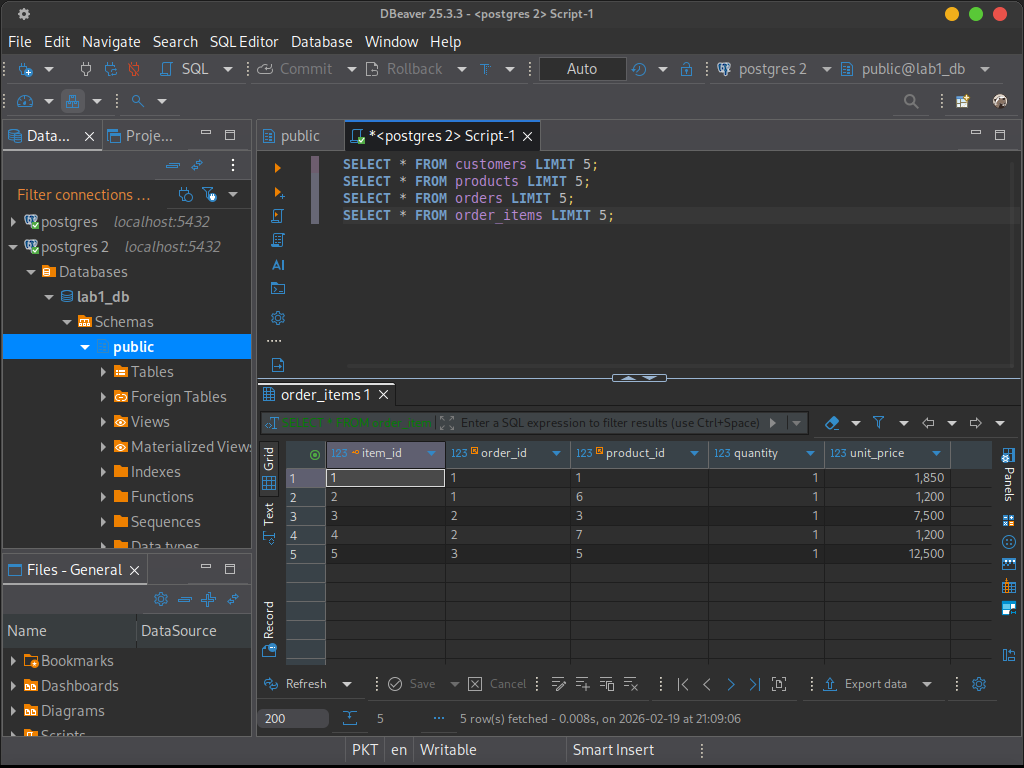
\includegraphics[width=0.95\textwidth]{EXPLORING-DATA.png}
\caption{Query 1: Exploring all four tables with LIMIT 5}
\label{fig:query1}
\end{figure}

\vspace{0.5cm}

% ============================================================================
% QUERY 2
% ============================================================================
\subsection{Query 2: Select Specific Columns}

\textbf{Objective:} Retrieve only customer name, city, and signup date, sorted by registration date.

\textbf{SQL Code:}
\begin{lstlisting}[language=SQL, style=SQL]
SELECT name, city, signup_date
FROM customers
ORDER BY signup_date;
\end{lstlisting}

\textbf{Explanation:}
\begin{itemize}
    \item Selects only 3 specific columns instead of all columns
    \item \texttt{ORDER BY signup\_date} sorts results chronologically (oldest first)
    \item Demonstrates column projection - selecting only needed data
    \item Results show customer growth over time (2023-2024)
\end{itemize}

\textbf{Alternative:} Using \texttt{ORDER BY signup\_date DESC} would show newest customers first.

\begin{figure}[H]
\centering
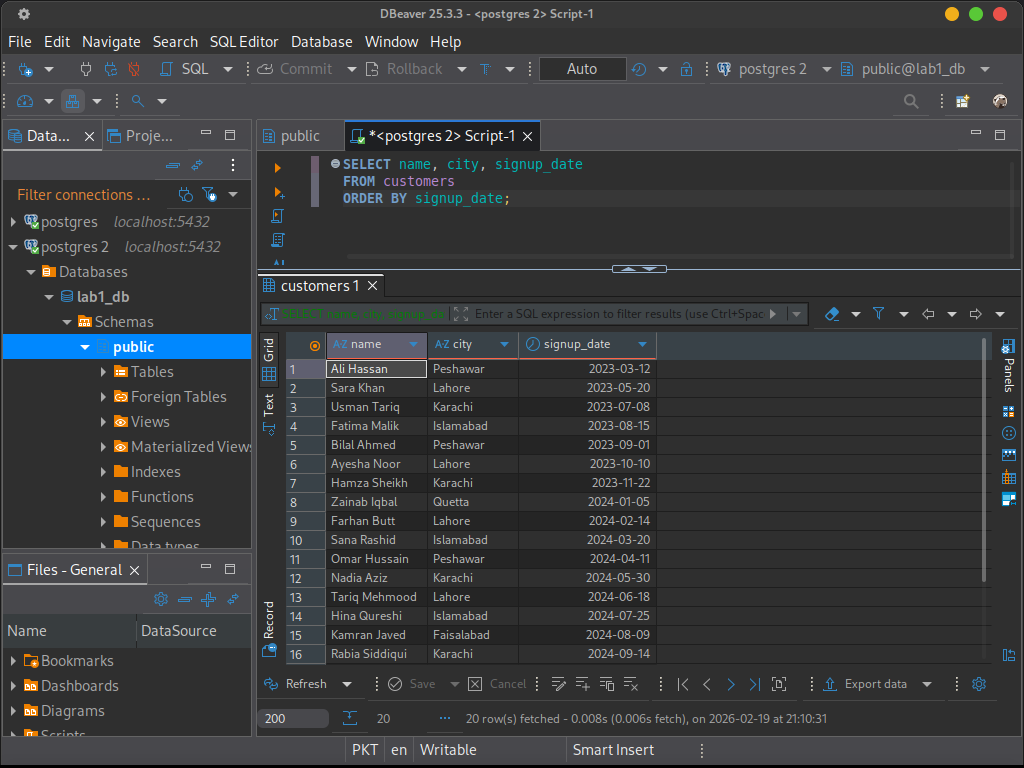
\includegraphics[width=0.95\textwidth]{Select-specific-columns.png}
\caption{Query 2: Customer names, cities, and signup dates sorted chronologically}
\label{fig:query2}
\end{figure}

\vspace{0.5cm}

% ============================================================================
% QUERY 3
% ============================================================================
\subsection{Query 3: Filter by Status}

\textbf{Objective:} Find all orders that have been delivered.

\textbf{SQL Code:}
\begin{lstlisting}[language=SQL, style=SQL]
SELECT order_id, customer_id, total_amount, order_date
FROM orders
WHERE status = 'delivered'
ORDER BY order_date DESC;
\end{lstlisting}

\textbf{Explanation:}
\begin{itemize}
    \item \texttt{WHERE status = 'delivered'} filters only completed orders
    \item \texttt{ORDER BY order\_date DESC} shows most recent deliveries first
    \item Demonstrates filtering with equality condition
    \item Useful for fulfillment tracking and delivery analytics
\end{itemize}

\textbf{Analysis:} By changing the status value to 'pending', 'processing', 'shipped', or 'cancelled', we can analyze order distribution across different statuses.

\begin{figure}[H]
\centering
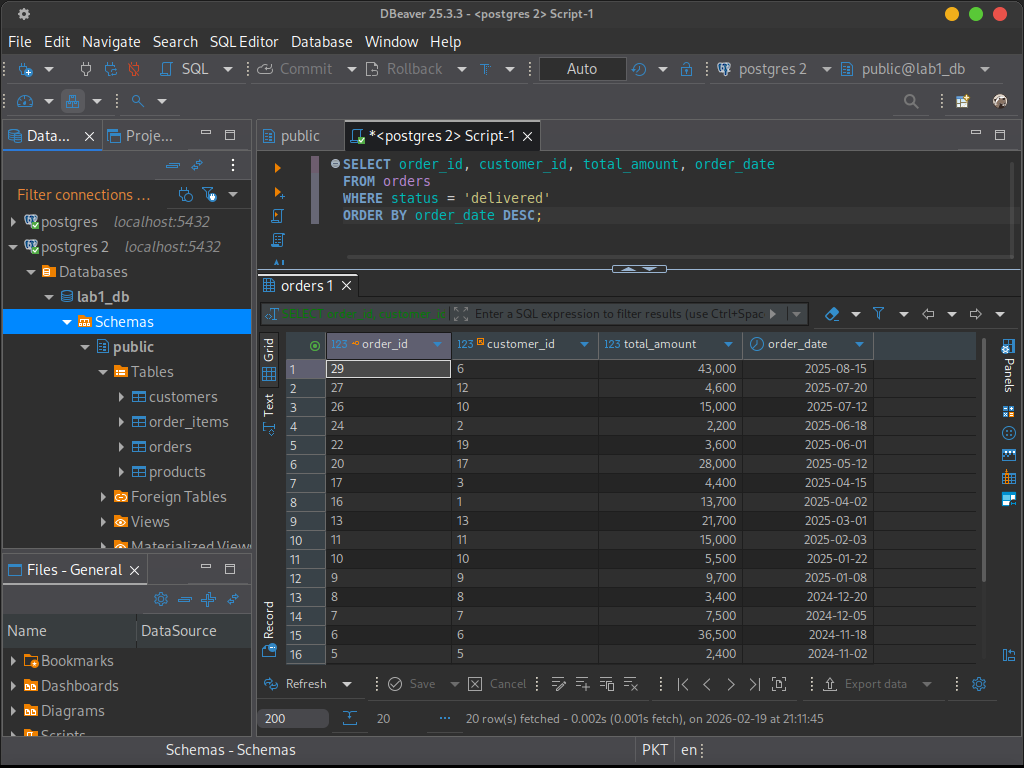
\includegraphics[width=0.95\textwidth]{Filter-by-status.png}
\caption{Query 3: All delivered orders sorted by date (newest first)}
\label{fig:query3}
\end{figure}

\vspace{0.5cm}

% ============================================================================
% QUERY 4
% ============================================================================
\subsection{Query 4: Filter by Price Range}

\textbf{Objective:} Find all products priced between 1,000 and 5,000 rupees using two different methods.

\textbf{SQL Code:}
\begin{lstlisting}[language=SQL, style=SQL]
-- Method A: BETWEEN operator
SELECT product_name, category, price
FROM products
WHERE price BETWEEN 1000 AND 5000
ORDER BY price;

-- Method B: Comparison operators
SELECT product_name, category, price
FROM products
WHERE price >= 1000 AND price <= 5000
ORDER BY price;
\end{lstlisting}

\textbf{Explanation:}
\begin{itemize}
    \item \textbf{Method A} uses \texttt{BETWEEN} - more concise and readable
    \item \textbf{Method B} uses explicit comparison operators - more flexible
    \item Both methods are \textbf{inclusive} (include boundary values 1000 and 5000)
    \item Both queries return identical results (9 products)
    \item Results sorted by price ascending
\end{itemize}

\textbf{Key Learning:} \texttt{BETWEEN X AND Y} is equivalent to \texttt{>= X AND <= Y}

\begin{figure}[H]
\centering
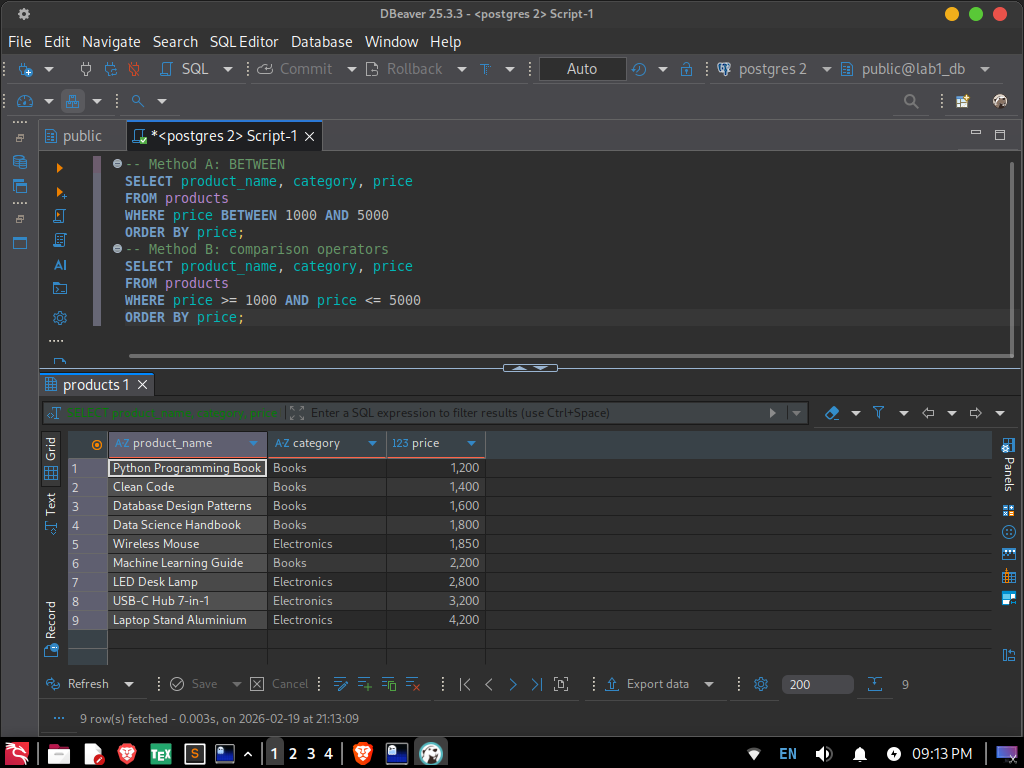
\includegraphics[width=0.95\textwidth]{Filter-by-price-range.png}
\caption{Query 4: Products priced between Rs. 1,000 and Rs. 5,000}
\label{fig:query4}
\end{figure}

\vspace{0.5cm}

% ============================================================================
% QUERY 5
% ============================================================================
\subsection{Query 5: Top 10 Highest-Value Orders}

\textbf{Objective:} Identify the 10 largest orders by total amount.

\textbf{SQL Code:}
\begin{lstlisting}[language=SQL, style=SQL]
SELECT order_id, customer_id, total_amount, status
FROM orders
ORDER BY total_amount DESC
LIMIT 10;
\end{lstlisting}

\textbf{Explanation:}
\begin{itemize}
    \item \texttt{ORDER BY total\_amount DESC} sorts highest values first
    \item \texttt{LIMIT 10} restricts to top 10 results
    \item Useful for identifying VIP customers and high-value transactions
    \item Important for fraud detection and revenue analysis
\end{itemize}

\textbf{Results Analysis:}
\begin{itemize}
    \item Highest order: Rs. 43,000 (order\_id 29)
    \item Top orders span different statuses (delivered, pending)
    \item Customer 6 appears twice in top 10 (loyal high-value customer)
\end{itemize}

\begin{figure}[H]
\centering
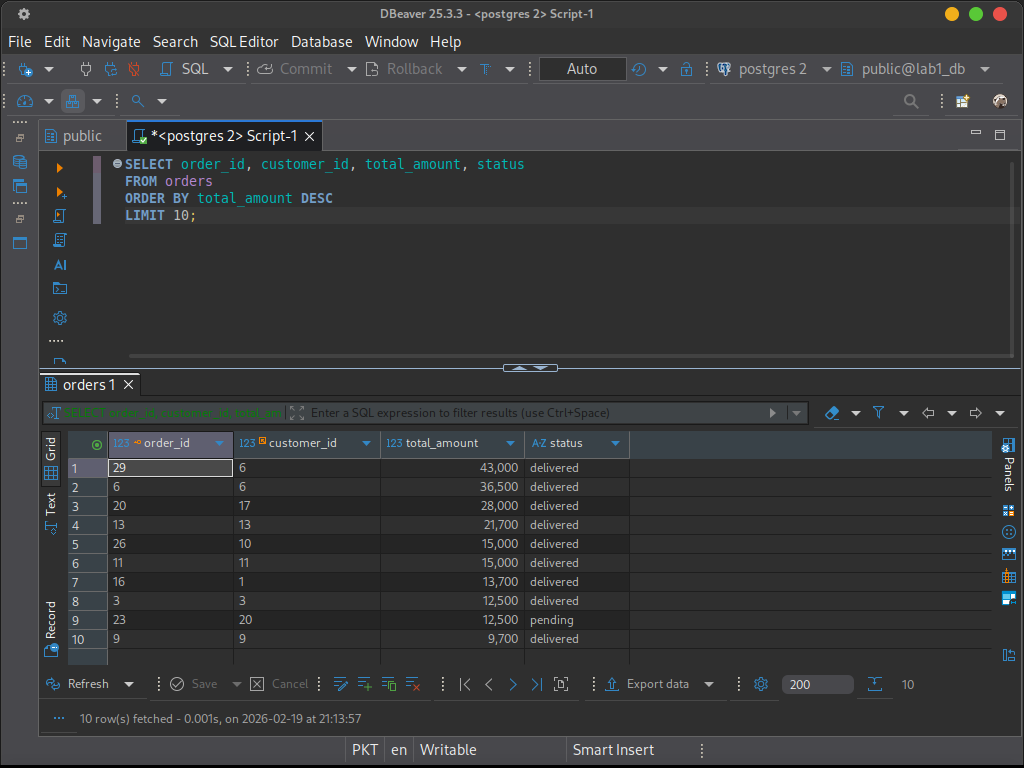
\includegraphics[width=0.95\textwidth]{Top-10-highest-value-orders.png}
\caption{Query 5: Top 10 orders by total amount (descending)}
\label{fig:query5}
\end{figure}

\vspace{0.5cm}

% ============================================================================
% QUERY 6
% ============================================================================
\subsection{Query 6: Multi-Condition Filter}

\textbf{Objective:} Find delivered orders from 2025 with total above Rs. 10,000.

\textbf{SQL Code:}
\begin{lstlisting}[language=SQL, style=SQL]
SELECT order_id, customer_id, total_amount, order_date
FROM orders
WHERE status = 'delivered'
  AND order_date >= '2025-01-01'
  AND total_amount > 10000
ORDER BY total_amount DESC;
\end{lstlisting}

\textbf{Explanation:}
\begin{itemize}
    \item Combines three conditions with \texttt{AND} operator
    \item Each condition on separate line for readability
    \item Filters by: status, date range, and monetary threshold
    \item Results sorted by value (highest first)
\end{itemize}

\textbf{Conditions Breakdown:}
\begin{enumerate}
    \item \texttt{status = 'delivered'} - Only completed orders
    \item \texttt{order\_date >= '2025-01-01'} - Orders from 2025 onwards
    \item \texttt{total\_amount > 10000} - High-value orders only
\end{enumerate}

\begin{figure}[H]
\centering
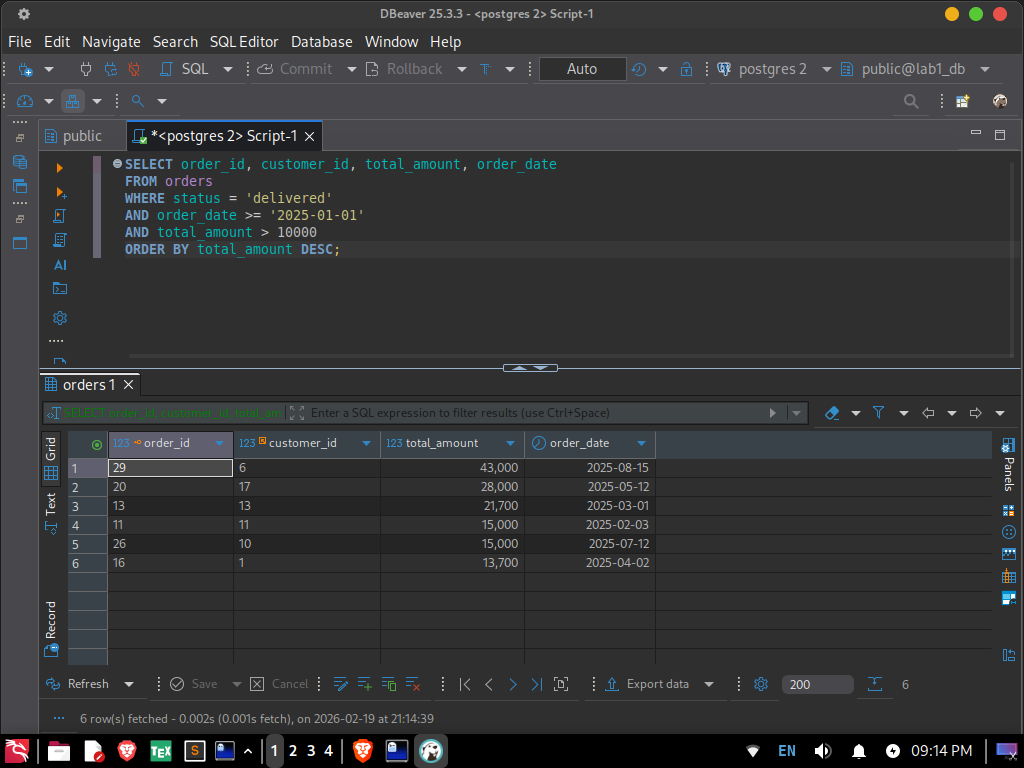
\includegraphics[width=0.95\textwidth]{Multi-condition-filter.png}
\caption{Query 6: Delivered orders from 2025 above Rs. 10,000}
\label{fig:query6}
\end{figure}

\vspace{0.5cm}

% ============================================================================
% QUERY 7
% ============================================================================
\subsection{Query 7: Pattern Matching on Email}

\textbf{Objective:} Find all customers with Gmail email addresses.

\textbf{SQL Code:}
\begin{lstlisting}[language=SQL, style=SQL]
SELECT name, email, city
FROM customers
WHERE email LIKE '%@gmail.com'
ORDER BY name;
\end{lstlisting}

\textbf{Explanation:}
\begin{itemize}
    \item \texttt{LIKE} operator enables pattern matching
    \item \texttt{\%@gmail.com} matches any text ending with @gmail.com
    \item \texttt{\%} is a wildcard matching zero or more characters
    \item Results sorted alphabetically by customer name
\end{itemize}

\textbf{Pattern Matching Variations:}
\begin{itemize}
    \item \texttt{LIKE '\%@yahoo\%'} - Find Yahoo users
    \item \texttt{LIKE 'a\%'} - Names starting with 'a'
    \item \texttt{ILIKE} - Case-insensitive version of LIKE
\end{itemize}

\textbf{Results:} 12 out of 20 customers (60\%) use Gmail addresses.

\begin{figure}[H]
\centering
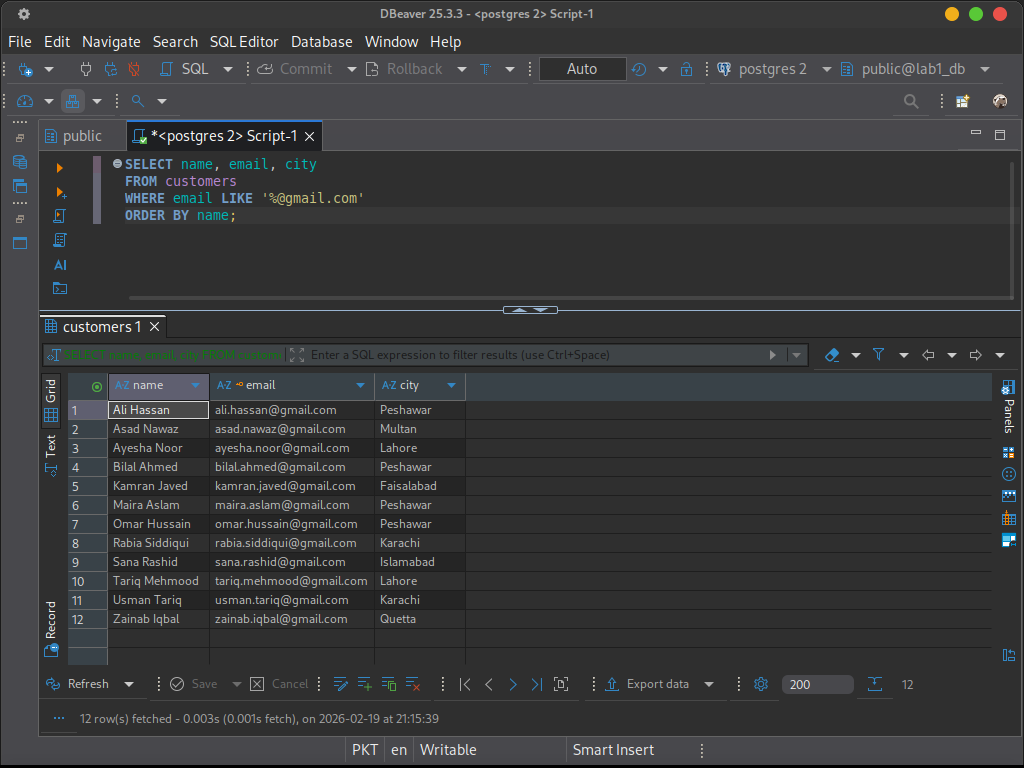
\includegraphics[width=0.95\textwidth]{Pattern-matching-on-email.png}
\caption{Query 7: Customers with Gmail email addresses}
\label{fig:query7}
\end{figure}

\vspace{0.5cm}

% ============================================================================
% QUERY 8
% ============================================================================
\subsection{Query 8: NULL Handling (Unshipped Orders)}

\textbf{Objective:} Find all orders that have not yet shipped (shipped\_date is NULL).

\textbf{SQL Code:}
\begin{lstlisting}[language=SQL, style=SQL]
SELECT order_id, customer_id, order_date, status, total_amount
FROM orders
WHERE shipped_date IS NULL
ORDER BY order_date;
\end{lstlisting}

\textbf{Explanation:}
\begin{itemize}
    \item \texttt{IS NULL} is the ONLY correct way to check for NULL values
    \item \texttt{= NULL} returns zero rows (silently wrong, not an error)
    \item NULL represents absence of value, not equal to anything
    \item Identifies orders pending shipment
\end{itemize}

\textbf{Important Concept:} NULL is not a value - it's the absence of a value. Nothing equals NULL, not even NULL itself.

\textbf{Results:} 7 unshipped orders found with statuses: pending, processing, cancelled.

\begin{figure}[H]
\centering
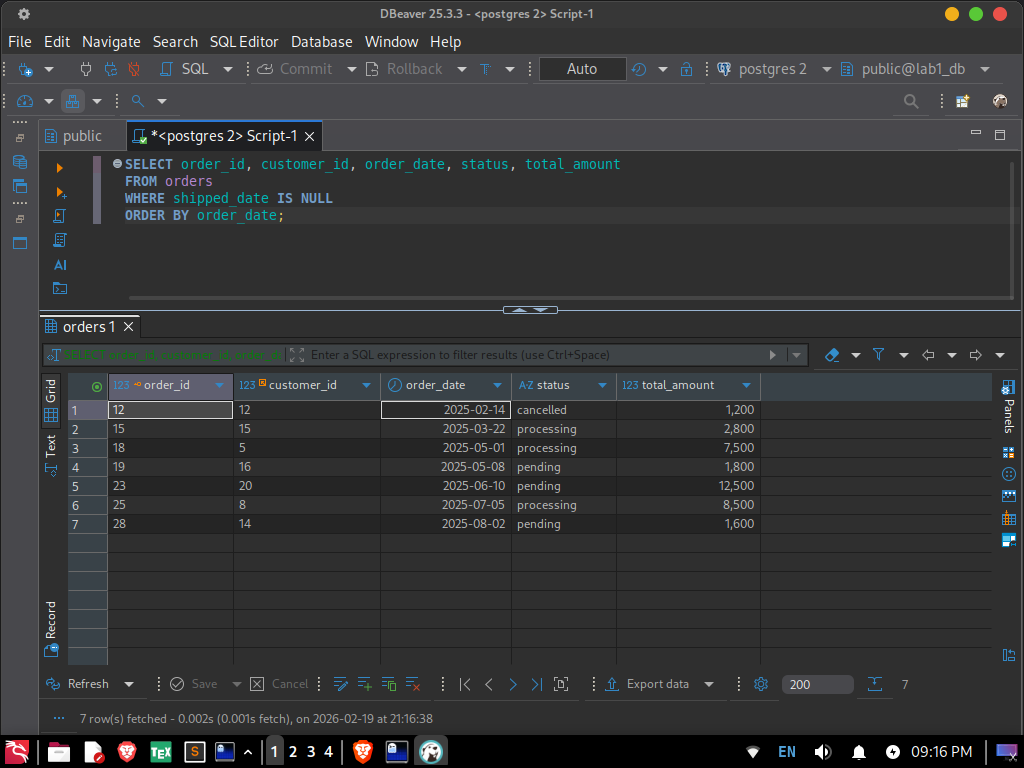
\includegraphics[width=0.95\textwidth]{NULL-handling-(unshipped-orders).png}
\caption{Query 8: Orders with NULL shipped\_date (not yet shipped)}
\label{fig:query8}
\end{figure}

\vspace{0.5cm}

% ============================================================================
% QUERY 9
% ============================================================================
\subsection{Query 9: Computed Column (Discount Calculation)}

\textbf{Objective:} Display products with original price, 20\% discounted price, and savings amount.

\textbf{SQL Code:}
\begin{lstlisting}[language=SQL, style=SQL]
SELECT product_name,
       category,
       price AS original_price,
       ROUND(price * 0.80, 2) AS discounted_price,
       ROUND(price * 0.20, 2) AS you_save
FROM products
ORDER BY discounted_price DESC;
\end{lstlisting}

\textbf{Explanation:}
\begin{itemize}
    \item Performs arithmetic directly in SELECT clause
    \item \texttt{price * 0.80} calculates 80\% of original (20\% discount)
    \item \texttt{price * 0.20} calculates savings amount
    \item \texttt{ROUND(value, 2)} rounds to 2 decimal places
    \item \texttt{AS} creates column aliases for readability
\end{itemize}

\textbf{Key Learning:} SQL can perform calculations on numeric columns without modifying stored data.

\begin{figure}[H]
\centering
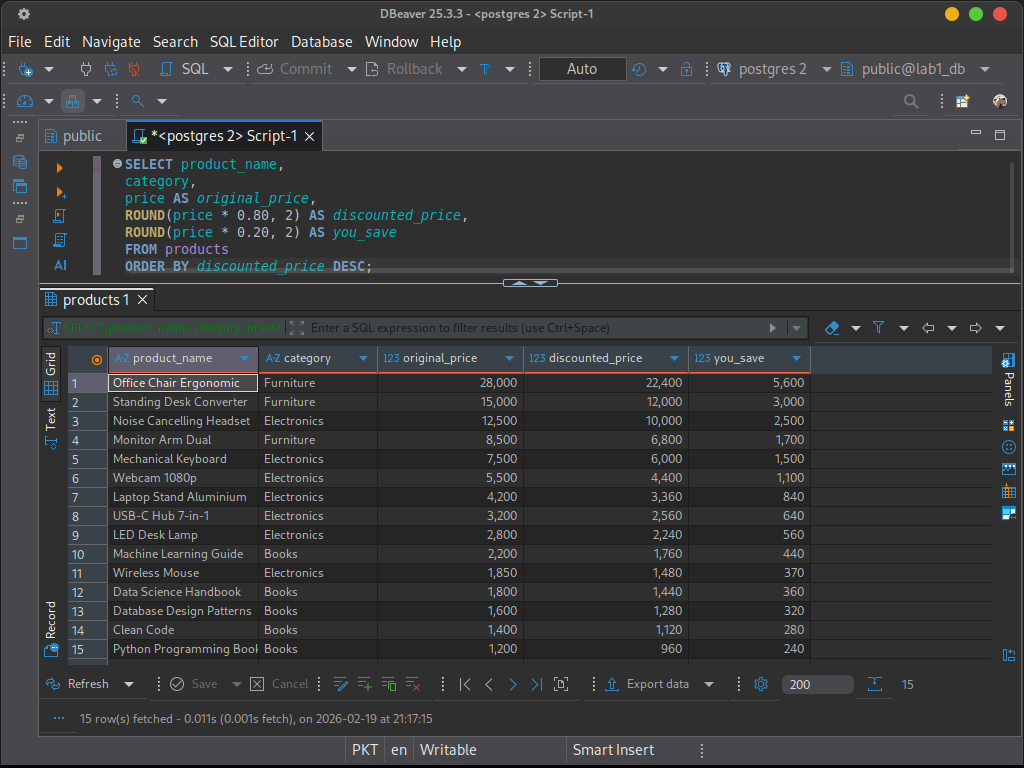
\includegraphics[width=0.95\textwidth]{Computed-column.png}
\caption{Query 9: Products with 20\% discount calculations}
\label{fig:query9}
\end{figure}

\vspace{0.5cm}

% ============================================================================
% QUERY 10
% ============================================================================
\subsection{Query 10: Bring Everything Together}

\textbf{Objective:} Find top 5 highest-value unshipped orders from 2025 with priority classification.

\textbf{SQL Code:}
\begin{lstlisting}[language=SQL, style=SQL]
SELECT order_id,
       customer_id,
       total_amount,
       order_date,
       status,
       CASE
           WHEN total_amount > 20000 THEN 'CRITICAL'
           WHEN total_amount > 5000 THEN 'URGENT'
           ELSE 'NORMAL'
       END AS priority
FROM orders
WHERE shipped_date IS NULL
  AND order_date >= '2025-01-01'
ORDER BY total_amount DESC
LIMIT 5;
\end{lstlisting}

\textbf{Explanation:}
\begin{itemize}
    \item \textbf{CASE WHEN} provides conditional logic (like if/else)
    \item Three-tier priority system: CRITICAL (>20k), URGENT (5k-20k), NORMAL (≤5k)
    \item Combines NULL handling, date filtering, and sorting
    \item Real-world application for order fulfillment prioritization
\end{itemize}

\textbf{CASE Expression Logic:}
\begin{enumerate}
    \item Check first WHEN condition - if true, return that value
    \item If false, check next WHEN condition
    \item If no conditions match, use ELSE value
\end{enumerate}

\textbf{Results:} Top unshipped order is Rs. 12,500 (URGENT priority).

\begin{figure}[H]
\centering
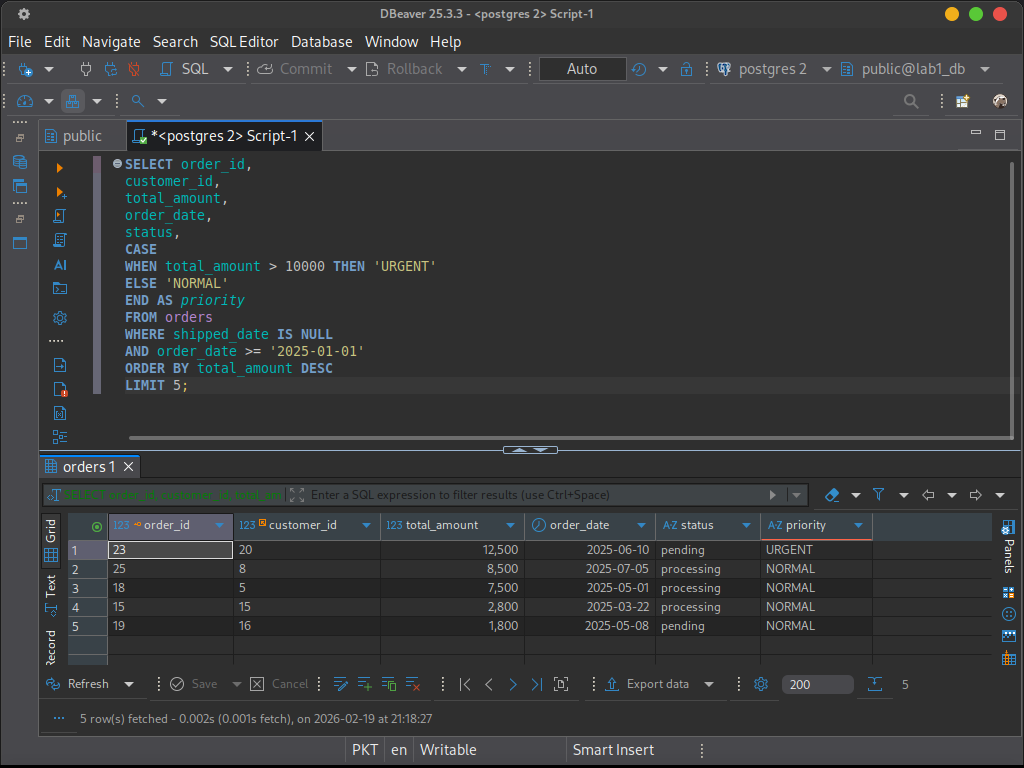
\includegraphics[width=0.95\textwidth]{Bring-everything-together.png}
\caption{Query 10: Top 5 unshipped 2025 orders with priority classification}
\label{fig:query10}
\end{figure}

\newpage

\section{Summary of SQL Concepts Learned}

\begin{table}[H]
\centering
\caption{SQL Concepts Covered in Lab 02}
\label{tab:concepts}
\begin{tabular}{@{}lll@{}}
\toprule
\textbf{Query} & \textbf{Primary Concept} & \textbf{Key Syntax} \\
\midrule
1 & Data Exploration & SELECT *, LIMIT \\
2 & Column Selection & SELECT col1, col2, ORDER BY \\
3 & Filtering & WHERE, equality condition \\
4 & Range Filtering & BETWEEN, comparison operators \\
5 & Sorting and Limiting & ORDER BY DESC, LIMIT \\
6 & Multi-Condition Filter & WHERE with AND \\
7 & Pattern Matching & LIKE, wildcards (\%) \\
8 & NULL Handling & IS NULL \\
9 & Computed Columns & Arithmetic, ROUND(), AS \\
10 & Conditional Logic & CASE WHEN, ELSE \\
\bottomrule
\end{tabular}
\end{table}

\section{Reflection}

This laboratory exercise reinforced fundamental SQL query writing skills through practical e-commerce scenarios. Key takeaways include:

\begin{itemize}
    \item \textbf{Tool Proficiency:} Gained experience with both DBeaver (GUI) and psql (CLI)
    \item \textbf{NULL Understanding:} Learned that NULL requires special handling with IS NULL
    \item \textbf{Pattern Matching:} Mastered LIKE operator with wildcards for text searches
    \item \textbf{Conditional Logic:} CASE WHEN enables complex business logic in queries
    \item \textbf{Code Readability:} Proper formatting and alignment improves query maintainability
\end{itemize}

Using both DBeaver and psql demonstrated why professional environments utilize both tools: DBeaver for visual analysis and quick exploration, psql for scripting and automation.

\vspace{0.5cm}
\noindent \textbf{GitHub Repository:} \url{https://github.com/Ayyankhan101/DATABASE-LAB.git}

\vspace{0.5cm}
\noindent \textbf{Files Created:}
\begin{itemize}
    \item \texttt{lab2/queries.sql} - All 10 SQL queries
    \item \texttt{lab2/ecommerce\_setup.sql} - Database schema and sample data
    \item \texttt{pdf2/lab02\_report.tex} - This LaTeX documentation
\end{itemize}

\end{document}
